\documentclass{article}

\usepackage[preprint, nonatbib]{neurips_2026}
\usepackage[utf8]{inputenc}
\usepackage[T1]{fontenc}
\usepackage{amsmath,amssymb,amsfonts}
\usepackage{nicefrac}
\usepackage{booktabs}
\usepackage{graphicx}
\graphicspath{{images/}}
\usepackage{hyperref}
\usepackage{url}
\usepackage{microtype}
\usepackage{xcolor}
\usepackage{enumitem}
\usepackage{array}
\usepackage{multirow}
\usepackage{tabularx}
\usepackage{verbatim}

\hypersetup{
  colorlinks=true,
  linkcolor=blue!60!black,
  citecolor=blue!60!black,
  urlcolor=blue!60!black,
}

\title{How LLM Agents Recover Trust:\\Empirical Verification Profiles and Concentration-Driven Scarring across Six Frontier Model Snapshots\thanks{Code, settings, raw logs, and analysis scripts: \url{https://github.com/cyjabc2020/Escape-room-v2}.}}

\author{
  Yujiao Chen \\
  Massachusetts Institute of Technology \\
  Cambridge, MA 02139 \\
  \texttt{yujiaoch@mit.edu}
}

\begin{document}

\maketitle

\begin{abstract}
Teams of AI agents are increasingly asked to work together, and doing so well requires each agent to judge how far to trust its partners. We study a simple but consequential version of that judgment: when a teammate makes a mistake early on but then becomes reliable, does an LLM agent forgive it, or does it keep double-checking that teammate long after the mistake? This matters because misjudging it is costly in both directions---persistent over-suspicion wastes effort and can make a team worse off, while too little caution lets real failures slip through.

We examine this in a cooperative survival game in which four agents must pool their answers to escape, and one teammate gives wrong answers in early rounds before becoming dependable. We vary which of six frontier model snapshots plays the trusting agent (Claude Opus 4.6, Claude Sonnet 4.6, GPT-5.1, GPT-5.4-mini, Gemini 3.1 Pro, Gemini 2.5 Flash) and how the unreliable teammate fails---a single early slip, or two failures either clustered together or spread apart---and we measure how much an agent keeps verifying the failed teammate (\emph{targeted caution}) versus the rest of the team (\emph{spillover distrust}).

Three findings emerge across 170 runs. First, recovery behavior is not a single pattern: runs fall into four empirically separable verification profiles. Second, what drives lasting suspicion is not how many times a teammate fails but whether those failures cluster together---in Claude Sonnet 4.6, two clustered failures leave a lasting scar $95\%$ of the time versus $40\%$ when the same two failures are spread out. Third, the two Anthropic snapshots show a sharp jump in scarring between one and two failures, with no further increase at three. We characterize these behaviors descriptively and do not claim that more or less verification is beneficial: whether scarring helps or harms a team depends on a task's payoff structure, which is outside our scope. All results are specific to the snapshots tested rather than to providers or model families in general.
\end{abstract}

%==============================================================================
\section{Introduction}
\label{sec:intro}
%==============================================================================

People who work in teams carry a running sense of who can be counted on. A colleague who fumbles an early task may find that others quietly double-check their work for weeks, long after they have become dependable. A little of this caution is prudent; too much is wasteful. The same tension is about to matter for AI agent teams, because we are increasingly handing coordination to teams of language-model agents \cite{park2023generative, hong2024metagpt, wu2023autogen}. When one agent's teammate slips early, does the agent forgive and move on, or does that early slip leave a lasting mark on how it treats the teammate from then on?

We call the lasting-mark version of this behavior \emph{trust scarring}: after a partner gives a wrong answer in a single early interaction, an agent keeps verifying that partner round after round, even once the partner has become consistently reliable. Scarring is not obviously a defect---some wariness after a failure is sensible---so the interesting questions are about its shape and its price. We ask three:

\begin{itemize}[leftmargin=*, itemsep=2pt, topsep=2pt]
  \item Does trust scarring generalize across most frontier model snapshots?
  \item What features of the failure sequence (count, timing, clustering) drive scarring?
  \item Does scarring produce better team outcomes, or does it carry costs?
\end{itemize}

We answer these in the Escape Room Survival Game, a cooperative multi-agent environment (Section~\ref{sec:env}), along two axes: cross-snapshot comparison across six specific frontier model releases (Section~\ref{sec:design}) and a \emph{D-failure schedule} axis manipulating the count, timing, and clustering of teammate failures while holding total failure count fixed.

\paragraph{Terminology.} We distinguish three levels of generality: a \emph{snapshot} is a specific dated model release (e.g., \texttt{gemini-3.1-pro-preview}); a \emph{model family} is a versioned series from one provider (e.g., Claude 4.6); a \emph{provider} is the company. Our findings are attributable to the specific snapshots tested, not to providers or families in general. When we discuss patterns shared by the two Anthropic snapshots we tested (Opus 4.6, Sonnet 4.6), we say so explicitly.

\paragraph{What we find.}
\begin{itemize}[leftmargin=*, itemsep=2pt, topsep=2pt]
  \item \textbf{H1: recovery is not one behavior.} When we group runs by how much an agent kept checking the failed partner versus the rest of the team, four distinct verification styles emerge, and the six snapshots spread across them in different ways.
  \item \textbf{H2: concentration matters more than count.} Two failures bunched together leave a far deeper scar than the same two failures spread across the game sequence.
  \item \textbf{H3: scarring switches on between one failure and two.} For the two Anthropic snapshots, going from one early failure to two sharply raises scarring; a third adds essentially nothing ($p=0.003$ for the one-to-two step, fixed-effects logistic regression).
\end{itemize}

We report these as descriptive characterizations of model behavior. We deliberately avoid claiming that scarring is beneficial or harmful: whether more verification helps a team is specific to a task's reward structure, which we do not vary here.

%==============================================================================
\section{Related Work}
\label{sec:related}
%==============================================================================

Our work sits at the meeting point of three lines of research.

\textbf{How people recover trust.} Behavioral economics and social psychology have long studied how trust is built and broken. Controlled trust games show that people extend and reciprocate trust at a personal cost \cite{berg1995trust} and will even pay to punish defectors in order to sustain cooperation \cite{fehr2002altruistic, axelrod1984evolution}. Yet trust is asymmetric: bad impressions weigh more heavily than good ones \cite{baumeister2001bad, slovic1993perceived}, and a violation is far easier to inflict than to repair \cite{schweitzer2006promises, kim2004removing}. Trust calibration is equally central to human--AI interaction, where a model's expressed confidence shapes how much users rely on it and how well they ultimately decide \cite{li2024miscalibrated}, and can even pull human self-confidence into alignment with the model's \cite{li2025confidence}. Trust scarring is, in effect, the machine analogue of these asymmetries, transposed to the agent--agent setting where one model must calibrate trust in another.

\textbf{Teams of LLM agents.} A fast-growing body of work puts LLM agents into cooperative and competitive settings \cite{park2023generative, hong2024metagpt, wu2023autogen, talebirad2023multi}, including repeated economic games \cite{akata2023repeated}, negotiation under conflicting interests \cite{bakhtin2022diplomacy}, and multi-agent debate in which agents cross-check one another's answers \cite{du2023debate, li2023camel}. These studies almost always examine a single model release, leaving open how behavior varies from one frontier snapshot to the next, and they rarely isolate how the \emph{timing} of a partner's failures shapes later trust.

\textbf{What we add.} A single-snapshot precursor documented trust scarring in GPT-5.1 \cite{chen2026trustfire}; building on it, we contribute three things: we compare behavior across six frontier snapshots rather than one; we manipulate \emph{when} and \emph{how} a partner fails, not just whether it fails; and we separate two kinds of suspicion---caution aimed at the culprit versus caution that spills onto innocent teammates.

%==============================================================================
\section{The Escape Room Survival Game}
\label{sec:env}
%==============================================================================

We need a setting where trust has teeth---where checking a teammate costs something and trusting a bad answer can be fatal---so that an agent's verification choices reveal what it actually believes about its partners. Our cooperative survival game provides this. Four agents (A, B, C, D) play a series of games, and the team escapes only when some agent \emph{volunteers} the correct, fully assembled four-part password. Each agent knows the answer to only its \emph{own} puzzle; for every other puzzle it sees only \emph{capsules}---public records that show the puzzle's index and the names of agents who have endorsed it, but never the answer inside. Each round an alive agent may \textbf{Pass}; \textbf{Verify} a puzzle, paying one coin to have that puzzle revealed to it alone so it can solve the puzzle itself---its answer then joins a matching capsule's endorser list, or opens a new capsule if it differs from all existing ones; or \textbf{Volunteer} a password, choosing which capsule to draw on for each slot when several exist. A correct volunteer lets the whole team---every agent still alive---escape together, with no special reward to the volunteer; an incorrect one kills the volunteer. If nobody volunteers, one agent is eliminated at random, so endless caution is itself dangerous. Each verification is thus a costly bet: an agent must judge, from endorsement patterns alone, which capsules to trust. Full mechanics are in Appendix~\ref{sec:appx-environment}.

\subsection{D-Failure Schedule}

To study trust recovery cleanly, we make one teammate's reliability fully scripted. Agent D is a deterministic stand-in that gives right or wrong answers according to a fixed schedule, so we control exactly when D fails and when it becomes dependable. By comparing schedules that differ in \emph{how many} times D fails and \emph{how those failures are spaced} (Table~\ref{tab:schedules}), we can ask not just whether an early failure scars, but which features of the failure---its count, its timing, its bunching---drive the scarring:

\begin{table}[h]
\centering
\caption{D-failure schedules (\textbf{T} = correct, \textbf{F} = incorrect). Perturbed cells (any schedule with at least one D-failure) run 11 games. Because D is correct throughout the smooth condition, the game count does not enter any failure-schedule contrast.}
\label{tab:schedules}
\small
\begin{tabular}{lll}
\toprule
Schedule & \texttt{correctness\_list} & Total D-failures \\
\midrule
smooth        & [T,\ldots,T] (all correct) & 0 \\
1-strike      & [F,T,T,T,T,T,T,T,T,T,T] & 1 (game 1) \\
2-strike      & [F,F,T,T,T,T,T,T,T,T,T] & 2 (games 1--2) \\
3-strike      & [F,F,F,T,T,T,T,T,T,T,T] & 3 (games 1--3) \\
mid2strike    & [T,T,T,F,F,T,T,T,T,T,T] & 2 (games 4--5; mid-game) \\
recur         & [F,T,T,T,F,T,T,T,T,T,T] & 2 (games 1 and 5; spread) \\
\bottomrule
\end{tabular}
\end{table}

\noindent The trick is the trio of 2-failure schedules. The 2-strike, mid2strike, and recur conditions all give D exactly two failures but place them differently---early and adjacent, mid-game and adjacent, or split far apart. Because the count is held fixed, any difference in scarring between them must come from timing and bunching rather than from sheer amount of evidence.

\subsection{Two Metrics of Trust Scarring}
\label{sec:metrics}

Once D has stopped failing, an agent's continued checking can point in two directions, and we track both. It can keep checking \emph{D specifically}---warranted-looking caution aimed at the teammate that actually slipped---or it can grow generally jumpy and check \emph{everyone}, including teammates who never did anything wrong. We call the first \emph{targeted caution} and the second \emph{spillover distrust}, and we measure them only in the games after D's last failure (e.g., games 4--11 for 3-strike). Since D is assigned the fourth puzzle, a \emph{Q4-verify} below is precisely a verification aimed at D. Per run:

\begin{itemize}[leftmargin=*, itemsep=1pt, topsep=2pt]
  \item \textbf{Targeted caution} $\mathrm{TARG} = \tfrac{\text{Q4-verify decisions}}{|G_{\text{post}}|}$ where $G_{\text{post}}$ is the set of games after the last D-failure.
  \item \textbf{Non-Q4 raw rate} $\mathrm{nonQ4} = \tfrac{\text{non-Q4-verify decisions}}{|G_{\text{post}}|}$.
  \item \textbf{Spillover distrust} $\mathrm{SPILL} = \mathrm{nonQ4} - \overline{\mathrm{nonQ4}}_{\text{smooth, same snapshot}}$.
\end{itemize}

We report both raw $\mathrm{nonQ4}$ and the normalized $\mathrm{SPILL}$ in Tables~\ref{tab:profiles} and~\ref{tab:clustering}. Table~\ref{tab:profiles} gives the cross-snapshot 1-strike summary used in the clustering analysis of Section~\ref{sec:h1}. A run is classified as \emph{scarred} if $\mathrm{TARG} > 0.5$. Scar proportions report Wilson 95\% confidence intervals; mean TARG and survival report normal 95\% CIs based on the sample SD with $n-1$ degrees of freedom. Threshold sensitivity is shown in Section~\ref{sec:threshold-sensitivity}.

%==============================================================================
\section{Experimental Design}
\label{sec:design}
%==============================================================================

\subsection{Model Snapshots}

We test six specific model snapshots, two per provider:

\begin{itemize}[leftmargin=*, itemsep=1pt, topsep=2pt]
  \item \textbf{OpenAI:} \texttt{gpt-5.1} and \texttt{gpt-5.4-mini-2026-03-17}, both at \texttt{reasoning\_effort="high"}.
  \item \textbf{Anthropic:} \texttt{claude-opus-4-6} and \texttt{claude-sonnet-4-6}, both at provider-recommended \texttt{thinking=\{"type":"adaptive"\}}.
  \item \textbf{Google:} \texttt{gemini-3.1-pro-preview} and \texttt{gemini-2.5-flash}, both at high thinking budget.
\end{itemize}

Exact snapshot identifiers, API routes, and decoding settings are in Appendix~\ref{sec:appx-repro}.

\paragraph{Data hygiene and sampling.} Runs are screened for contamination before analysis using two complementary mechanisms. First, to catch transient API failures, an automatic filter scans each run's agent-reasoning and decision text for provider error markers (overload, rate-limit, and service-degradation responses captured as ERROR strings). Second, to catch degenerate runs in which a provider returned near-empty or truncated completion, we apply an outcome-integrity inspection to filter anomalously high defaulted-to-pass decision rates. From the screened pool we standardize sampling by keeping the earliest completed runs by timestamp, with a target of $n=10$ per perturbed cell (any schedule in which D fails at least once) and $n=5$ per smooth baseline cell. This yields $\mathbf{170}$ runs across 20 cells, with every cell at its target $n$.

%==============================================================================
\section{Results}
\label{sec:results}
%==============================================================================

\subsection{H1: Four Empirical Clusters in (TARG, SPILL) Space}
\label{sec:h1}

Start with the simplest case: a single early failure (the 1-strike schedule), seen across all six snapshots (Table~\ref{tab:profiles}). Even here there is no single ``recovery behavior.'' Some snapshots barely react---GPT-5.4-mini keeps checking the failed partner only $0.46$ times per later game and scars in $3$ of $10$ runs---while Gemini Flash reacts hard, checking the partner more than once per game on average and scarring in $9$ of $10$. The snapshots also differ in \emph{where} their caution lands: Sonnet actually checks the rest of the team \emph{less} than at baseline after D fails (SPILL $=-0.21$), focusing its attention narrowly, whereas Gemini Pro becomes broadly more suspicious (SPILL $=+1.37$).

\begin{table}[h]
\centering
\caption{Cross-snapshot 1-strike recovery scarring. SPILL is computed relative to same-snapshot smooth baseline. Scar rate uses Wilson 95\% CI; TARG and survival use normal 95\% CI.}
\label{tab:profiles}
\small
\begin{tabular}{lrlcclc}
\toprule
Snapshot & $n$ & TARG [95\% CI] & non-Q4 raw & SPILL & Scar rate [Wilson 95\% CI] & Survival \% \\
\midrule
\texttt{gpt-5.1} (Replicate)             & 10 & 0.56 [0.32, 0.80] & 0.62 & $+0.26$ & 4/10 = 40\% [17, 69]  & 91.4 \\
\texttt{claude-opus-4-6}                 & 10 & 0.52 [0.20, 0.84] & 1.59 & $+0.05$ & 5/10 = 50\% [24, 76]  & 91.4 \\
\texttt{claude-sonnet-4-6}               & 10 & 0.54 [0.14, 0.94] & 1.65 & $-0.21$ & 3/10 = 30\% [11, 60]  & 87.3 \\
\texttt{gpt-5.4-mini-2026-03-17} (high)  & 10 & 0.46 [0.15, 0.77] & 1.86 & $+0.69$ & 3/10 = 30\% [11, 60]  & 78.2 \\
\texttt{gemini-3.1-pro-preview}          & 10 & 0.76 [0.46, 1.06] & 2.00 & $+1.37$ & 7/10 = 70\% [40, 89]  & 80.2 \\
\texttt{gemini-2.5-flash}                & 10 & 1.12 [0.83, 1.41] & 4.05 & $+0.48$ & 9/10 = 90\% [60, 98]  & 45.2 \\
\bottomrule
\end{tabular}
\end{table}

To see whether these differences form a few recognizable styles rather than a continuum, we let the data group itself. Placing every recovery run at its (targeted caution, spillover distrust) coordinates and running $k$-means clustering ($k \in \{2,\dots,6\}$ on the 140 runs with a usable smooth baseline), the cleanest grouping is into four clusters: the silhouette score peaks at $k=4$ ($0.530$), and the four-way split is stable under bootstrap resampling (mean ARI $0.90$; Fig.~\ref{fig:clustering}). In other words, the messy spread of behaviors resolves into four recurring verification styles.

\begin{figure}[h]
\centering
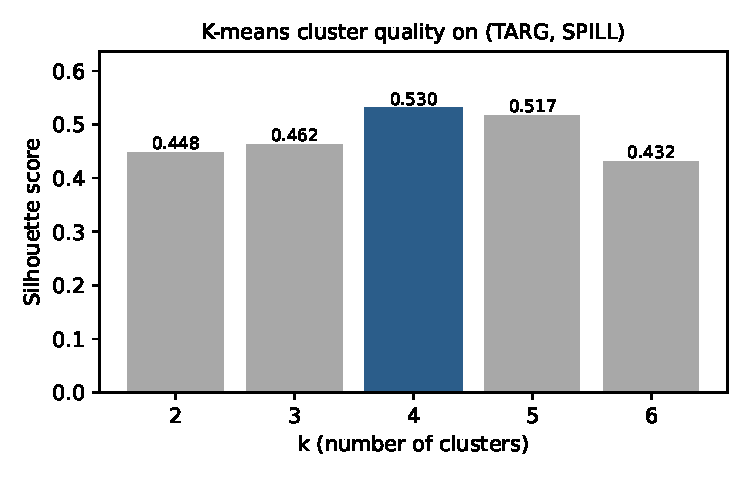
\includegraphics[width=0.32\textwidth]{clustering_silhouette.pdf}
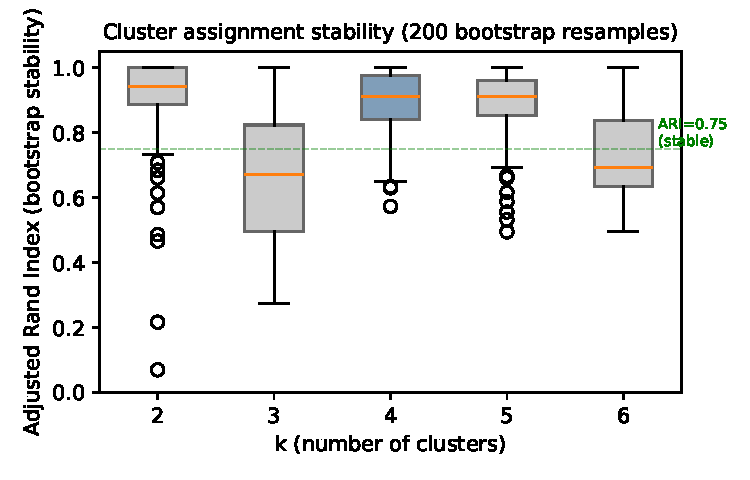
\includegraphics[width=0.32\textwidth]{clustering_bootstrap.pdf}
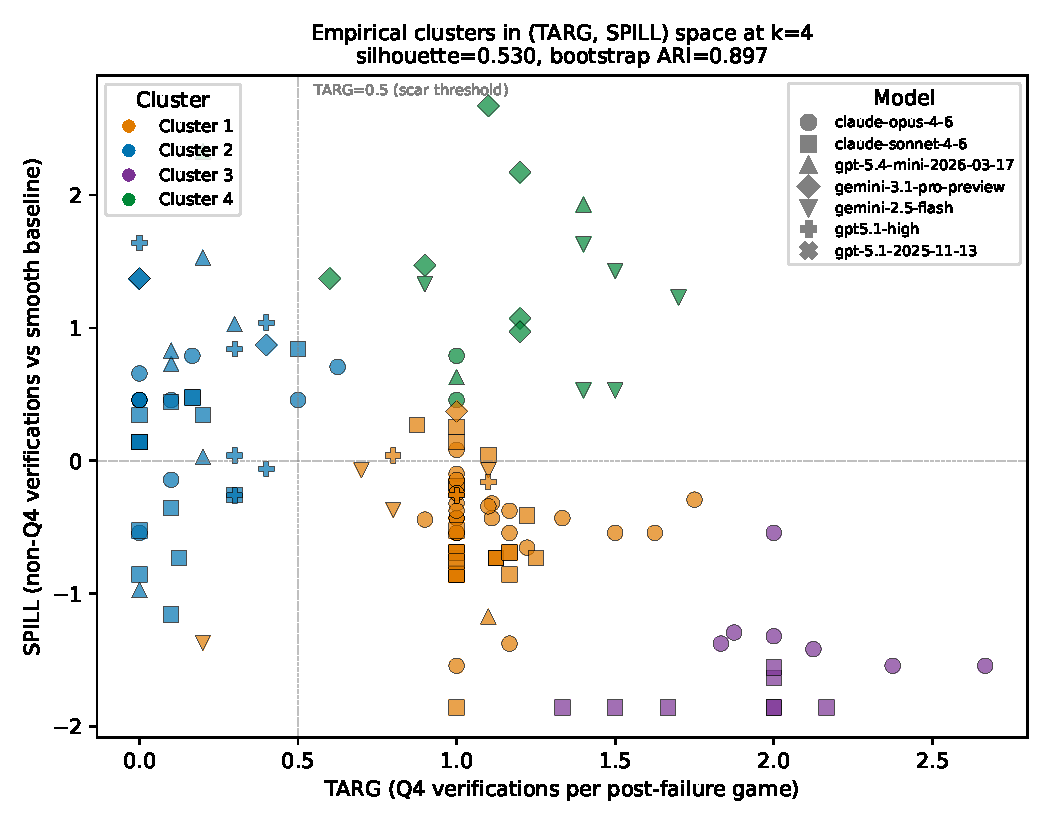
\includegraphics[width=0.34\textwidth]{clustering_scatter.pdf}
\caption{$k$-means clustering analysis on standardized (TARG, SPILL) features.
Left: silhouette score by $k$ (peak at $k=4$).
Middle: bootstrap Adjusted Rand Index ($200$ resamples; the $k=4$ split is stable, mean ARI $0.90$).
Right: scatter plot of all $n=140$ perturbed runs in (TARG, SPILL) space, colored by cluster assignment at $k=4$; markers indicate snapshot.}
\label{fig:clustering}
\end{figure}

The four styles have intuitive characters (centroids in raw units; full composition in Appendix~\ref{sec:appx-clusters}):

\begin{itemize}[leftmargin=*, itemsep=1pt, topsep=2pt]
  \item \textbf{Moderate surgical} (Cluster 1; TARG=$1.05$, SPILL=$-0.51$, $n=65$): keeps a steady eye on the culprit while easing off everyone else. This is the most common style by far, and the one most Anthropic multi-strike runs fall into.
  \item \textbf{Mild caution} (Cluster 2; TARG=$0.15$, SPILL=$+0.34$, $n=43$): barely singles out the culprit and stays only slightly more watchful overall---essentially ``recovered.'' Drawn from single-failure and spread-out-failure runs across many snapshots.
  \item \textbf{Extreme surgical} (Cluster 3; TARG=$1.97$, SPILL=$-1.56$, $n=15$): an intense, laser-focused fixation on the culprit paired with the lowest checking of everyone else. This corner is entirely Anthropic, led by Opus 3-strike and Sonnet 2-strike.
  \item \textbf{High targeting, high spillover} (Cluster 4; TARG=$1.13$, SPILL=$+1.33$, $n=17$): suspicious of the culprit \emph{and} the whole team---the ``paranoid'' style---dominated by Gemini Flash and Pro.
\end{itemize}

We treat these as empirical styles, not fixed ``provider traits.'' The four groupings themselves are stable under resampling, but which style a given snapshot lands in depends on the specific snapshots and failure schedules we tested, and should not be read as a permanent property of any model.

\paragraph{Method robustness.} The cluster structure is robust to clustering method choice. Re-running with hierarchical (Ward and average linkage) yields Adjusted Rand Index of $0.72$ and $0.88$ respectively against $k$-means (Appendix~\ref{sec:appx-cluster-robustness}). The $k$-means silhouette is the highest among the methods tried ($0.53$ vs $0.45$ for Ward), consistent with the empirical points being approximately spherically distributed around their cluster centroids. We caution that with only two dimensions (TARG, SPILL) and $n=140$ runs, the cluster structure is necessarily coarse; a richer feature set (per-game decision diversity, survival, decision timing) could reveal finer structure but would inflate the dimensionality beyond what our sample size supports.

\paragraph{Snapshot-level mapping to clusters.} Across the recovery family, Anthropic snapshots populate Clusters 1 and 3 (the surgical clusters) predominantly; Google snapshots populate Cluster 4 predominantly; OpenAI snapshots (GPT-5.1 and Mini) populate Clusters 1 and 2. This mapping is a description of the data we have, not a prediction about untested snapshots.

\subsection{H3: Scarring Switches On Between One Failure and Two}
\label{sec:h3}

A single slip seems to be forgivable, but a second one changes things. For both Anthropic snapshots, the scar rate is moderate after one failure and near-total after two, then flat at three (Table~\ref{tab:threshold}): Opus jumps from $50\%$ to $100\%$, Sonnet from $30\%$ to $90\%$. It is as though one mistake reads as bad luck while two read as a pattern---and once the pattern is established, a third failure adds little.

\begin{table}[h]
\centering
\caption{Anthropic count progression. Wilson 95\% CI on scar rate; normal 95\% CI on TARG.}
\label{tab:threshold}
\small
\begin{tabular}{lcll}
\toprule
Snapshot \& Schedule & $n$ & TARG [95\% CI] & Scar rate [Wilson 95\% CI] \\
\midrule
\multicolumn{4}{l}{\emph{Claude Opus 4.6 (Adaptive thinking)}}\\
\quad smooth   & 5  & 0.17 [0.12, 0.23] & 0/5 = 0\% [0, 43] \\
\quad 1-strike & 10 & 0.52 [0.20, 0.84] & 5/10 = 50\% [24, 76] \\
\quad \textbf{2-strike} & \textbf{10}  & \textbf{1.18 [0.99, 1.37]} & \textbf{10/10 = 100\% [72, 100]} \\
\quad 3-strike & \textbf{10}  & 1.54 [1.17, 1.90] & \textbf{10/10 = 100\% [72, 100]} \\
\midrule
\multicolumn{4}{l}{\emph{Claude Sonnet 4.6 (Adaptive thinking)}}\\
\quad smooth   & 5  & 0.43 [0.03, 0.82] & 2/5 = 40\% [12, 77] \\
\quad 1-strike & 10 & 0.54 [0.14, 0.94] & 3/10 = 30\% [11, 60] \\
\quad \textbf{2-strike} & \textbf{10}  & \textbf{1.22 [0.83, 1.61]} & \textbf{9/10 = 90\% [60, 98]} \\
\quad 3-strike & 10  & 0.96 [0.77, 1.16] & 9/10 = 90\% [60, 98] \\
\bottomrule
\end{tabular}
\end{table}

A logistic regression confirms the jump and the plateau. Fitting \emph{scarred} on schedule (relative to 1-strike, controlling for snapshot, across all $n=140$ perturbed runs), the move to two adjacent failures is large and significant ($\beta = +3.37$, $95\%$ CI $[+1.17, +5.58]$, $p=0.003$), and the move to three lands at exactly the same coefficient ($\beta = +3.37$, $p=0.003$)---no further amplification. Crucially, the two spread-out schedules move the needle far less: a mid-game pair raises scarring modestly (mid2strike $\beta = +1.81$, $p=0.013$) and two failures split far apart are statistically indistinguishable from one (recur $\beta = +0.61$, $p=0.34$). So the action is in the step from one \emph{adjacent} failure to two, not in piling on more.

\subsection{H2: Concentration, Not Just Count, Drives Scarring}
\label{sec:h2}

This is the most striking result in the paper. Fix the number of failures at exactly two and vary only their spacing, and the depth of scarring swings dramatically. Table~\ref{tab:clustering} shows the effect in Sonnet, where it is largest; Opus moves in the same direction (Appendix~\ref{sec:appx-clustering-opus}).

\begin{table}[h]
\centering
\caption{Clustering effect in \texttt{claude-sonnet-4-6} at fixed 2 D-failures.}
\label{tab:clustering}
\small
\begin{tabular}{lcllc}
\toprule
Condition & $n$ & TARG [95\% CI] & Scar rate [Wilson 95\% CI] & non-Q4 (raw) \\
\midrule
2-strike (clustered early)    & 10 & 1.22 [0.83, 1.61] & 9/10 = 90\% [60, 98] & 0.91 \\
mid2strike (clustered mid)    & 10 & \textbf{1.23 [1.00, 1.46]} & \textbf{10/10 = 100\% [72, 100]} & 0.92 \\
\textbf{clustered combined} (2-strike $+$ mid2strike) & \textbf{20} & 1.23 [1.01, 1.45] & \textbf{19/20 = 95\% [76, 99]} & 0.91 \\
recur (spread)                & 10 & 0.52 [0.13, 0.90] & \textbf{4/10 = 40\% [17, 69]} & 1.50 \\
\bottomrule
\end{tabular}
\end{table}

The same two D-failures, distributed differently across an 11-game sequence, produce substantially different scar rates: $19/20 = 95\%$ when the two failures are clustered (whether early or mid-game) versus $4/10 = 40\%$ when spread. Fisher's exact test for the clustered-versus-spread contrast gives $p = 0.002$ (clearly significant). The Wilson 95\% CIs for clustered (76--99\%) and spread (17--69\%) are non-overlapping. The fixed-effects logistic regression places recur on essentially the same statistical footing as 1-strike ($\beta = +0.61$ vs reference, $p=0.34$), while the two clustered schedules are both elevated ($\beta = +3.37$ for 2-strike and $+1.81$ for mid2strike).

Critically, the spread condition (recur) trains the model with \emph{more recent} evidence of D-unreliability than the early-clustered condition (the second failure occurs at game 5 vs game 2 in 2-strike), yet produces less scarring. This is not well explained by naive monotonic evidence accumulation; richer accounts (recency-weighted, salience-thresholded, or memory-compressed accumulators) could in principle produce this pattern.

The mid2strike condition---failures after 3 games of established reliability---produces Sonnet's highest scar rate (10/10 = 100\%), consistent with a violation-of-expectation interpretation: failures against an established baseline of reliability are more readily encoded as a pattern.

%==============================================================================
\section{Statistical Robustness}
\label{sec:robustness}
%==============================================================================

\subsection{Threshold Sensitivity}
\label{sec:threshold-sensitivity}

Our headline scar rate uses the threshold $\mathrm{TARG} > 0.5$ to classify a run as scarred. We sweep this threshold from $0.3$ to $0.8$ and verify that the qualitative findings are robust (Fig.~\ref{fig:threshold}).

\begin{figure}[h]
\centering
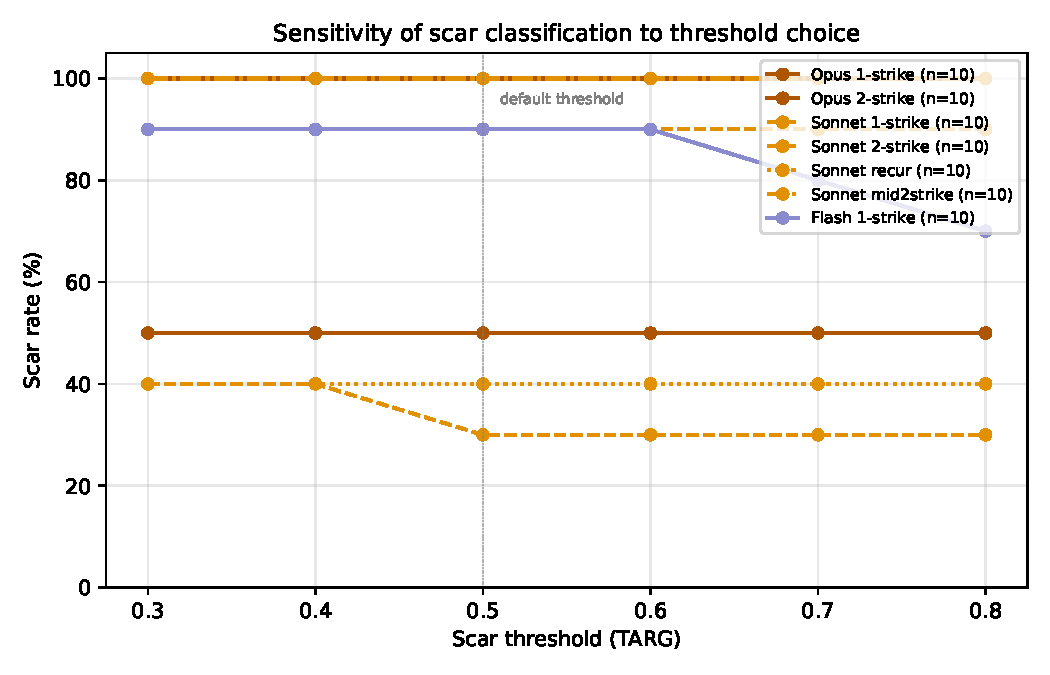
\includegraphics[width=0.7\textwidth]{scar_threshold_sensitivity.pdf}
\caption{Sensitivity of scar classification to threshold choice. Lines connect (threshold, scar rate) pairs per cell. Headline contrasts (Sonnet recur vs 2-strike; Opus 1-strike vs 2-strike) are robust over the swept range.}
\label{fig:threshold}
\end{figure}

\subsection{Pairwise Tests with Multiple-Comparison Correction}

We ran 15 pairwise comparisons across the cells of interest (cross-family at 1-strike; within-Anthropic count progression; within-Anthropic clustering manipulation). Fisher's exact tests on proportions and Mann--Whitney $U$ tests on TARG were Benjamini--Hochberg corrected across the 15-test family. Full table in Appendix~\ref{sec:appx-pairwise}.

No pairwise contrast survives BH correction at our current $n$ (all BH-adjusted $p > 0.05$ across the 15-test family); the fixed-effects logistic regression reported in Section~\ref{sec:h3} provides more powerful inference by pooling across cells. We report both.

%==============================================================================
\section{Discussion}
\label{sec:discussion}
%==============================================================================

\paragraph{What explains the cluster differences across snapshots?} Without intervention on model internals, we can only correlate. The clusters we observe correlate with each snapshot's smooth-baseline verification rate: snapshots with high baselines (e.g., Flash, $\overline{\mathrm{nonQ4}}=3.57$ per game) populate the high-SPILL cluster (Cluster 4); snapshots with low baselines (GPT-5.1, $\overline{\mathrm{nonQ4}}=0.36$) tend toward lean targeted scarring (Cluster 1). Anthropic snapshots show an intermediate baseline (Opus $\sim 1.54$, Sonnet $\sim 1.86$) that combines with their adaptive thinking mode to produce reduced non-Q4 verification under recovery (Cluster 3 in extreme cases). These are post-hoc correlations, not mechanism claims.

\paragraph{Why would spacing matter so much?} We can only speculate, but one possibility is appealing. An agent's memory across games is carried by a running summary in words, not by a running tally of probabilities. Two failures sitting side by side are easy to compress into a single story---``D is unreliable''---while two failures separated by stretches of good behavior never quite cohere into one. On this view a scar is less a count of evidence than a narrative that did or did not form. We cannot test this directly here, but it fits the pattern: the spread-out schedule actually gives the agent \emph{more recent} evidence of failure, yet scars least.

\paragraph{Cross-snapshot vs cross-family claims.} Our findings are attributable to the six specific snapshots tested. The cluster mapping ``Anthropic snapshots populate Clusters 1 and 3'' is a description of our data; we do not extrapolate to untested Claude versions. The clustering analysis and its stability are however robust to bootstrap resampling, which gives some confidence the structure is not an artifact of any single snapshot's runs.

\paragraph{What this means for building agent teams.} Different snapshots recover trust in markedly different ways, and how concentrated a partner's failures are strongly shapes the response. Which model suits a given deployment therefore depends on the failure patterns it is likely to encounter. We deliberately stop short of recommending more or less verification: whether continued checking helps or hurts a team is a function of the task's payoff structure---here, the specific coin, verification, and elimination economics---which we hold fixed and do not vary, so we make no general claim that scarring is beneficial or harmful.

\subsection{Limitations}
\label{sec:limits}

\begin{itemize}[leftmargin=*, itemsep=1pt, topsep=2pt]
  \item \textbf{Within-cell variance.} Cells are modest in size---$n=10$ for each perturbed cell and $n=5$ for each smooth baseline. We use Wilson CIs and a pooled fixed-effects logistic regression to handle the resulting uncertainty, but the per-cell confidence intervals remain wide and no pairwise comparison survives Benjamini--Hochberg correction at this sample size.
  \item \textbf{Snapshot specificity.} All claims are tied to the snapshot identifiers in Table~\ref{tab:repro-snapshots}.
  \item \textbf{Task simplicity.} Puzzles are single- and two-digit arithmetic. Whether the concentration finding transfers to richer task domains is open.
  \item \textbf{Fixed-strategy dummy.} D is a deterministic responder. Future work should test against partners whose reliability is updated by interaction.
  \item \textbf{Payoff-specific consequences.} Whether scarring benefits or harms a team depends on the task's reward structure (the coin, verification, and elimination economics used here). We characterize behavior, not its desirability, and make no general claim that trust scarring is good or bad.
\end{itemize}

%==============================================================================
\section{Conclusion}
\label{sec:conclusion}
%==============================================================================

Trust recovery in these agents is not one thing. Across six frontier snapshots in a controlled cooperative game, how an agent treats a teammate after an early failure splits into four recognizable styles---from near-complete forgiveness, to a laser fixation on the culprit, to broad and indiscriminate suspicion---and which style appears depends on the snapshot.

One pattern cuts across those differences: what cements a scar is not how \emph{often} a teammate fails but whether its failures \emph{cluster}. Two adjacent slips leave a deep mark where the same two, spread apart, largely wash out, and for the Anthropic snapshots the decisive step is from the first failure to the second.

We report these results for the specific snapshots we tested, and offer them as a starting map of a behavior that will only matter more as agents increasingly work in each other's company. We characterize how these agents recover trust, not whether their caution is well-calibrated: whether more or less verification helps a team is a payoff-dependent question we leave open.

%==============================================================================
\bibliographystyle{plain}
\bibliography{references}

\appendix

%==============================================================================
\section{Reproducibility Appendix}
\label{sec:appx-repro}
%==============================================================================

\subsection{Model Snapshots and API Access}

\begin{table}[h]
\centering
\caption{Exact model snapshots, API routes, and access dates.}
\label{tab:repro-snapshots}
\small
\begin{tabular}{lllc}
\toprule
Provider & Snapshot ID & API route & Access window \\
\midrule
OpenAI    & \texttt{openai/gpt-5.1} & Replicate & 2026 \\
OpenAI    & \texttt{gpt-5.4-mini-2026-03-17} & Direct OpenAI & 2026 \\
Anthropic & \texttt{claude-opus-4-6} & Direct Anthropic & 2026 \\
Anthropic & \texttt{claude-sonnet-4-6} & Direct Anthropic & 2026 \\
Google    & \texttt{gemini-3.1-pro-preview} & Direct Google & 2026 \\
Google    & \texttt{gemini-2.5-flash} & Direct Google & 2026 \\
\bottomrule
\end{tabular}
\end{table}

\subsection{Decoding Settings}

\begin{itemize}[leftmargin=*, itemsep=1pt, topsep=2pt]
  \item \textbf{OpenAI snapshots:} \texttt{reasoning\_effort="high"} for both GPT-5.1 and Mini; \texttt{max\_completion\_tokens=16384} for reasoning calls, $50$ for verifier sub-tasks. Temperature is silently ignored by these reasoning models.
  \item \textbf{Anthropic snapshots:} \texttt{thinking=\{"type":"adaptive"\}} for agent decision calls; no thinking parameter on verifier sub-tasks. \texttt{max\_tokens=16384} thinking-enabled / $50$ verifier.
  \item \textbf{Google snapshots:} \texttt{gemini-3.1-pro-preview} at default thinking level; \texttt{gemini-2.5-flash} with \texttt{thinking\_budget=-1} (dynamic) on decision calls and \texttt{thinking\_budget=0} (disabled) on verifier sub-tasks.
\end{itemize}

\subsection{Metric Implementation and Raw Logs}

Per-rep metric extraction is implemented in \texttt{code/scripts/compute\_metrics.py}; clustering in \texttt{clustering\_analysis.py}; statistical tests in \texttt{statistical\_models.py}; paper figures in \texttt{paper\_figures.py}. All scripts consume the canonical \texttt{per\_rep\_metrics.csv} file. Raw per-game JSON logs and decision CSVs are available at the linked repository under \texttt{code/results/}, one folder per run with a timestamp suffix.

\section{Environment Details}
\label{sec:appx-environment}

The game proceeds in rounds with four agents (A, B, C, D). Each agent is privately assigned one of the four puzzles---a short arithmetic question---and knows the question (and hence the answer) only for its own puzzle. For every other puzzle, an agent can see neither the question nor any answer directly; it sees only \emph{capsules}.

\paragraph{Capsules.} A capsule is a public record for a single puzzle that displays (i) the puzzle's index and (ii) the list of agents who have endorsed it. Crucially, the answer held inside a capsule is \emph{not} visible: an agent can see \emph{who} has vouched for a puzzle, but not \emph{what} they vouched for. Multiple capsules may coexist for the same puzzle index when agents have arrived at different answers.

\paragraph{Actions.} Each round, every alive agent simultaneously chooses one of:
\begin{itemize}[leftmargin=*, itemsep=1pt, topsep=2pt]
  \item \textbf{Pass}: take no action.
  \item \textbf{Verify}($j$): pay one coin to have puzzle $j$ revealed---only to that agent, and only for that moment---and solve it independently. If the agent's answer matches an existing capsule for puzzle $j$, its name is added to that capsule's endorser list; if the answer differs from every existing capsule, a new capsule is created with that answer and the agent as its sole endorser.
  \item \textbf{Volunteer}: submit a full four-part password, choosing for each slot which capsule's answer to use when more than one capsule exists. A correct submission lets all surviving agents escape; an incorrect one kills the volunteering agent.
\end{itemize}

If no alive agent volunteers in a round, one alive agent is eliminated uniformly at random, so indefinite caution is itself fatal. Each agent begins with a pool of coins that funds verification, and team survival is measured as the fraction of agents alive at game end. Agents A, B, and C are the LLM snapshot under test; agent D is a scripted responder whose answers are correct or incorrect according to the D-failure schedule (Table~\ref{tab:schedules}), the only experimental manipulation on this base game.

\section{Per-Cluster Composition (k=4)}
\label{sec:appx-clusters}

\begin{table}[h]
\centering
\small
\caption{Number of runs per (snapshot, schedule) in each cluster.}
\begin{tabular}{lcccc}
\toprule
& Cluster 1 & Cluster 2 & Cluster 3 & Cluster 4 \\
& moderate & no scar, & extreme & high targeting, \\
& surgical & mild caution & surgical & high spillover \\
\midrule
TARG centroid & 1.05 & 0.15 & 1.97 & 1.13 \\
SPILL centroid & $-0.51$ & $+0.34$ & $-1.56$ & $+1.33$ \\
\midrule
Total $n$ & 65 & 43 & 15 & 17 \\
\bottomrule
\end{tabular}
\end{table}

Top contributors by cluster:
\begin{itemize}[leftmargin=*, itemsep=1pt, topsep=2pt]
  \item Cluster 1 (moderate surgical, $n=65$, most populated): Opus 2-strike (9), Sonnet 3-strike (9), Sonnet mid2strike (7), Opus recur (6), Sonnet 2-strike (6), Opus 1-strike (5), Opus 3-strike (4), Opus mid2strike (4), Flash 1-strike (4), GPT-5.1 1-strike (4), Sonnet recur (3), plus scattered 1-strike runs.
  \item Cluster 2 (mild caution, $n=43$): Sonnet 1-strike (7), Sonnet recur (6), Mini 1-strike (6), Opus 1-strike (5), GPT-5.1 1-strike (6), Opus mid2strike (4), Opus recur (3), Pro 1-strike (3), and single Opus 3-strike / Sonnet 2-strike / Sonnet 3-strike runs.
  \item Cluster 3 (extreme surgical, $n=15$): all-Anthropic high-strike scarring corner --- Opus 3-strike (4), Sonnet 2-strike (3), Sonnet mid2strike (3), and single runs from Opus 2-strike/mid2strike/recur and Sonnet 1-strike/recur.
  \item Cluster 4 (high targeting, high spillover, $n=17$): Gemini Flash 1-strike (6), Gemini Pro 1-strike (6), Mini 1-strike (3), plus single Opus 3-strike and Opus mid2strike runs.
\end{itemize}

\section{Opus Clustering Effect (Companion to Section~\ref{sec:h2})}
\label{sec:appx-clustering-opus}

\begin{table}[h]
\centering
\caption{Clustering effect in \texttt{claude-opus-4-6} at fixed 2 D-failures.}
\small
\begin{tabular}{lcllc}
\toprule
Condition & $n$ & TARG [95\% CI] & Scar rate [Wilson 95\% CI] & non-Q4 (raw) \\
\midrule
2-strike    & 10 & 1.18 [0.99, 1.37] & 10/10 = 100\% [72, 100] & 1.06 \\
3-strike    & 10 & 1.54 [1.17, 1.90] & 10/10 = 100\% [72, 100] & 1.05 \\
mid2strike  & 10 & 0.87 [0.38, 1.36] & 6/10 = 60\% [31, 83] & 1.28 \\
recur       & 10  & 0.85 [0.45, 1.25] & 7/10 = 70\% [40, 89] & 1.15 \\
\bottomrule
\end{tabular}
\end{table}

For Opus the clustering effect is in the same direction as Sonnet's but smaller in magnitude. Recur and mid2strike both produce mixed outcomes (6--7 of 10 scarred) while 2-strike and 3-strike are unambiguous (10/10).

\section{Pairwise Comparison Table}
\label{sec:appx-pairwise}

The complete pairwise comparison table with Fisher's exact tests on scar rates, Mann--Whitney $U$ tests on TARG, Cohen's $h$ and $d$ effect sizes, and Benjamini--Hochberg corrected $p$-values is provided in \texttt{code/scripts/pairwise\_table.csv}. Of 15 comparisons, several pass the unadjusted threshold ($p < 0.05$) but none survive the multi-test correction, which is conservative at the current sample sizes. The fixed-effects logistic regression reported in Section~\ref{sec:h3} pools power across cells and reports the central count-threshold effect with $p = 0.003$ after the regression's standard-error treatment.

\section{Clustering Method Robustness (Companion to Section~\ref{sec:h1})}
\label{sec:appx-cluster-robustness}

To test robustness of the $k=4$ result, we ran two alternative clustering methods on the same standardized (TARG, SPILL) feature space, all with $k=4$:

\begin{itemize}[leftmargin=*, itemsep=1pt, topsep=2pt]
  \item \textbf{$k$-means (reference):} silhouette $0.530$.
  \item \textbf{Hierarchical (Ward linkage):} silhouette $0.453$, ARI = $0.724$.
  \item \textbf{Hierarchical (average linkage):} silhouette $0.510$, ARI = $0.875$.
\end{itemize}

$k$-means produces the highest silhouette, indicating that the clusters are best described as spherical around their centroids; the alternative methods that allow more flexible cluster shapes find similar global structure (substantial ARI agreement) but with worse silhouette. We interpret this as: the underlying cluster structure is method-robust at the level of identifying which broad regions of the (TARG, SPILL) plane are populated, but individual point assignments at cluster boundaries are method-dependent.

\section{Recommended Replication Designs}
\label{sec:appx-future}

\subsection{Cell Completion and Scaling}

All cells are now at their sampling target ($n=10$ for perturbed cells, $n=5$ for smooth baselines). The remaining limitation is statistical power, not coverage: the within-cell variance in several conditions (especially Opus mid2strike at $\mathrm{SD}=0.95$ on TARG) reflects genuine run-level bimodality rather than measurement noise, so increasing $n$ to $20$ for the borderline cells would tighten Wilson CIs from $\pm \sim 30\%$ to $\pm \sim 20\%$ and bring the primary pairwise tests closer to BH-survivable significance under reasonable effect sizes.

\end{document}
